\documentclass[Journal, InsideFigs, DoubleSpace]{ascelike} %NewProceedings, Journal

%\usepackage{endfloat}

%include package for inserting picture
\usepackage{graphicx}%insert image
\DeclareGraphicsExtensions{.pdf,.png,.jpg}
\graphicspath{{figures/}}%folder contains images

\usepackage{caption}%packages for inserting multiple pictures
\usepackage{subcaption}%packages for inserting multiple pictures

\usepackage{array}%for table with fixed width
\newcolumntype{L}[1]{>{\raggedright\let\newline\\\arraybackslash\hspace{0pt}}m{#1}}
\newcolumntype{C}[1]{>{\centering\let\newline\\\arraybackslash\hspace{0pt}}m{#1}}
\newcolumntype{R}[1]{>{\raggedleft\let\newline\\\arraybackslash\hspace{0pt}}m{#1}}

\usepackage{amsmath} %math package

\usepackage{algorithm} %algorithm package
\usepackage[noend]{algpseudocode} % pseudo code package

\usepackage[utf8]{inputenc}%french accents
\usepackage[T1]{fontenc} %for accented characters

%\usepackage[linesnumbered,ruled]{algorithm2e} %algorithm package

\usepackage{booktabs}%allowing drawing hline in table in some columns only


\begin{document}

% TITLE AND AUTHORS
\title{Automatic generation of civil engineering lexicon to support natural language based data retrieval}

%
\author{
Tuyen Le
\thanks{
Ph.D. Student, Department of Civil, Construction and Environmental Engineering, Iowa State University. Ames, IA 50011, United States. E-mail: ttle@iastate.edu.},
\and
H. David Jeong
\thanks{Associate Professor, Department of Civil, Construction and Environmental Engineering, Iowa State University. Ames, IA 50011, United States. E-mail: djeong@iastate.edu.}
 }
%MAKE TITTLE
\maketitle
%
\begin{center}
(To be submitted to the Journal of Computing in Civil Engineering) 
\end{center}
%ABSTRACT
\begin{abstract} %150-175 words (as required by ASCE)
Digital datasets are presented only in computer-readable formats and they are mostly complicated. In order to accurately extract a required subset of data, end users need to have deep understanding of the structure of the data schema, the meaning of each data entity and a query language. Thus, to truly facilitate the reuse of digital project data, a computational platform is needed to allow users to present their data needs in natural language. One of the critical requirements for a computer to perform this task is the ability to understand and interpret users' natural language inputs where keywords are a basic linguistic component. This research aims to collect technical terms commonly used in the civil infrastructure domain and develop a semantic similarity model that can measure the meaning relatedness/similarity between terms. Natural Language Processing (NLP) techniques and C-value method are used to automatically extract terms from text documents. A machine learning model called Skip-gram model is then employed to learn the semantic relatedness between technical terms using the unlabeled highway corpora as the input data. The input corpus includes over 15 million words mainly collected from roadway design guidelines across the U.S. The model is evaluated by comparing the mapping results performed by a computer and a human. 
\end{abstract}
%KEYWORDS
\KeyWords{Civil infrastructure project, Landxml, Data retrieval, Natural language interface, NLP, Vector space model}
%
%\newpage


%********************************************************
%good terms and phrases:

%adj: nonhierarchical, superior, well-defined; foreseeable; rigid, flexible, empirical, disparate, isolated, 

%sentence strucutre:  this is evidenced by the accelerating emergence of ...; 

%noun: challenges, barrier, hinders, obstacles, impediment; that approximate concepts; extraction=deduction=acquisition; broad spectrum; overtake these technical and economic challenges; bottleneck; data crreation and utilization; in the midst of planning; interpretation; 

%verb: emcombass; tackle, foster, amplified; simplified; detect; aggregate; 

%sentence template: tailored with respect to their context; includes three phases, namely AA, BB and CC; at such places as parks, fairgounds or town spuares; case-specific developments; area of interests; incrementally built; inexpensive and easy-to-use testing device; time and cost-efficient way; research community; one of..since then is the; RDF structure..to make assertion about a resource; syntax-centered NLP;  such as A, B, etc.; ..is in it's reliance upon the presence..which is..; with the objectives of disambiguation; has triggered a mounting awareness; to be the main impediment to the progess; ..start point for deducing other truth; lastly; there is a large body of research on; see e.g. [2], [14] and [32]; the former, the latter; rigorously formalized; backbone strucutre of st; was opted to; Sections 4.5 and 4.6; (e.g., Neo4J, OrientDB, Titan); forthcoming year; well-designed process; is subject to do st; in turn means that; discussion by academics and professionals; some insights on planning, management, and control; strategic framework; in-depth project performance; in lieu of; 

%term': empirical work; linguistic unit/term; 

%axiomatic richness, formality of representation,  

%the following expression denotes, is presented/defined as follows, this/below example shows, the snippet below presents, the following is the short description of the rule, an OWL ontology describing an ifcwindow class, these concepts and relationships can be encoded in the following RDF/XML fragment, is written in Turtle syntax/format:
%The tool is meant to assess, 
%********************************************************

%BODY
\section{Introduction}%900 words
%research background, structured data vs unstructure data: easily to for searching, to be searched
%Topic introduction, territory: centrality--> genearal background information 
Neutral data standards have been widely accepted as the solution to the interoperability issue in the construction industry. Several open standards have been proposed, ranging from solely relying on syntactics using Express Modeling Language such as Industry Foundation Classes (IFC) \cite{buildingsmartIFC} or LandXML \cite{landxmlorg} to semantics-rich ontologies such as e-COGNOS \cite{Lima05}. These standardized data models consist of rich sets of data elements covering various business processes and disciplines. However, since a specific data exchange scenario needs only a subset of data, hence neutral data standards alone are insufficient to facilitate seamless digital data exchange among project stakeholders \cite{Froese03,east12}. As querying data on those data schema which are large and complicated the end user is required to have considerable programming skills and properly understand the structure and the meaning of each entity or attribute included in the source data schema. Data driven decision making based on a wrong extracted dataset would likely lead to a wrong decision. Therefore, there is a need for the formal definitions of schema subsets determining the right data for specific transactions. The availability of these model views will underpin the extraction of data from complicated sets of data generated from the AEC industry. 
\par
%Identify the niche: overall to one aspect to be addressed--> limitation in current state -->highlight the problem, raise general questions, propose general hypotheses --> emphasize the need (justify the need to address)
%niche #1: state of practices-a reliance on human-crafted work
The MVD development is a process of matching required data items for a specific domain to the data names in the neutral data schema. A considerable amount of research efforts has been made in both the building and transportation sectors with the same ambition to define subsets of data for various business processes. One of these efforts is the Construction to Operation Building Information Exchange (Cobie) project \cite{east07} which is now becomes a part of a variety of national standards and guidelines for projects using Building Information Modeling (BIM), for instance UK COBie 2.4 \cite{nisbet12}, National BIM Standard-United States Version 3 (NBIMS-US) \cite{nibs15}, GSA-BIM Guide \cite{gsa11}. This research identified IFC data elements that are generated in the design and construction phases required to be transferred to the asset management phase. The civil sector also is going on this trend with several model views of the Landxml schema has been being defined. The examples of these include the InfraModel project carried by the Technical Research Center of Finland aims to specify subsets of LandXML schema for several transportation projects and this specification has become the Finish national application specification \cite{inframodel14}. Even though a considerable number of research have been made, but these are still limited to a large demand from the industry. This is because the current method for developing model view definition is based on a manual basic which is time consuming \cite{venugopal12,eastman12,hu14}. The business processes are dynamic and tend to change over time. To adapt to the changes from industry practices, these model view are required to be tailored. Therefore, there is a need to change the current practice of model view definition from the ad-hoc approach to a more rigorous methodology \cite{venugopal12}. 
\par
%niche: the importance of dictionaries, ontologies to text analysis, mining and the shortage of dictionaries in civil industry
In this task, NLP techniques, text based ontology learning methods and the proposed vector space model in task 2 will be utilized to construct a highway machine-readable dictionary. The dictionary will organize terms in a lexical hierarchy through semantic relations such as synonym, attribute, hyponym and hypernym. Since this knowledge base is represented in a machine readable manner, it allows for the automation of variety of knowledge works such as reasoning for code compliance checking or constructability review, information retrieval, and word sense disambiguation in digital data exchange. However, like other domains, the highway industry stores knowledge in text documents which are readable to only human. This task aims to transform highway domain knowledge in natural language into a machine-readable format.
\par
%niche #2: challenge to the automated process
In order to eliminate the human-reliance MDV procedure, the automated method and tool are demanded. Those program needs to automatically match user data needs to the data labels in the the integrated data space. Using keywords to extract data from a database is more favorable to the end user thanks to the ease of use. This can properly done without mismatching if computer can understand the meaning of user requirements instead of string sequence based matching. Technical keywords/terms in domain specific documents implicitly refer to something that only expert in that field can correctly understand. For example, the term roadway type, in general context it can be a classification system of roadway in terms of material, function, location, etc. But in the highway context, it refers to roadway functional classification. Another example about the use of different terms for the same thing is that the 'vertical alignment' which is the long section and is the longitudinal centerline of road way have variety of terminology including 'profile', 'crest', 'grade-line'. Different DOTs may have their own vocabulary system that usually attached as glossary in their documents. different terms may be used to describe about the same thing (many different way to describe the same thing). In this case, computer is unable to to exact to map term between data sender and data receiver during the data exchange process if the algorithm is only relying on the data label/name.  Due to this reason the current practices of MDV generation are still a manual process.
\par
% potential tools and method to address the above issue
Recent advances in computer science with considerable improvements have enabled computer to understand human-readable format. This is thanks to the achievement in semantic measure related research which provide infrastructure for computer to present technical keywords in numeric format which can be understood by computer. A large number of methods have been proposed ranging from statistical method to machine learning such as. Distributional model is one of the most common and has been widely used. These achieve high accuracy. The availability of these offer potentials tools for the construction industry to enhance the manual work matching technical keywords in a specific domain to the open data schema. 
\par
%Objectives (research goals, questions/hypotheses, methodology, and main results) --> claiming the value of the research --> outline the structure of the paper
To fill the gap above, this research aims to propose a novel model that can be used to measure the semantic similarity between technical terms in the civil infrastructure domain. In order to achieve that goal, Natural Language Processing (NLP) techniques and C-Value method [9] are employed to process domain-specific guidelines and extract technical terms commonly used in the civil sector. A matching algorithm implementing the result from the previous step is developed to automatically look for the most nearest entities and attributes in the Landxml schema for a certain keyword. The proposed semantic similarity model and the data mapping algorithm are evaluated by comparing the automatic retrieved data with the manual results from a human for performance assessment.. The framework was complied into a Java package and full lexicon datasets which is available at https://github.com/tuyenbk/mvdgenerator.
%
\section{Related research} \label{sec:litrev} %2000 words
%section introduction
This research employed a hybrid approach which combines a series of techniques related to text analysis and semantic similarity measurement to semantically match user's input keywords to the data entities in the sources schema. Each technique is meant to support each phase of the proposed methodology. The details of research methodology will be presented in the section \ref{sec:proposed_method} below. This section presents a the state-of-the-art regarding partial model extraction in the construction industry and a brief introduction to the techniques deployed in the research framework.


\subsection{Semantic data label matching}

%ontology matching
In current practices, data input to support a certain data analytics process usually come from multiple resources. These data are stored in different formats and are based upon different vocabularies systems. These inconsistency restricts the ability of data integration and likely leads to semantic ambiguities. In the ontology based data integration and exchange mechanism, ontology serves as a domain data schema. To allow for data exchange or integration, target and source ontology are required to  be matched to each other. Matching is the process of find corresponding relationships (e.g. sameAS, isA, etc.) among semantic entities (concept, words, sentences, instances, etc.) between these ontologies \cite{harispe15}. These relations are found thanks to the semantic measures which determine the degree of relatedness between concepts \cite{harispe15}. 

\subsubsection{Lacking of an extensive machine-readable dictionary for the civil infrastructure domain}
Digital dictionaries, which present definitions of terms in a machine-readable manner, are critical for computer to perform knowledge works such as interpreting users’ intention or understanding the meaning behind human-oriented inputs. However, there is still a shortage of such an extensive dictionary for the civil engineering domain. WordNet (Miller 1995) \cite{miller95}, which is one of the largest lexicons with over 117,000 synsets, is still generic and not suitable for the highway domain. A few construction domain specific semantic resources have been proposed, for example the Civil Engineering Thesaurus (CET) (Abuzir and Abuzir 2002) \cite{abuzir02}, e-Cognos (Wetherill et al. 2002) \cite{wetherill02}, and buildingSMART data dictionary (ISO 12006-3) (buildingSMART 2016)\cite{buildingsmartData} . Of these knowledge bases, the buildingSMART dictionary is a pioneer semantic database with a long development history of over two decades by the international collaboration of buildingSMART Norway, Construction Specifications Canada (CSC), U.S. Construction Specification Institute (CSI), and STABU Foundation (Hezik 2008) \cite{hezik08}. Like other construction specific digital dictionaries, IFD is mainly hand-coded and time consuming; the vocabulary set covers limited number of concepts. Therefore, there is a demand for a computational technique that can automatically develop and maintain these digital dictionaries to keep up with the increasingly arising of new terms. 
%
\subsubsection{Lacking of effective semantic mapping algorithms for handling the data ambiguity issue}
%Other academic research on semantic mapping
In the construction industry, research efforts are currently focusing on standardizing the data structure format, there are few research have been done to deal with the issue of sense ambiguity. Zhang and El-Gohary (2015) \cite{Zhang15c} proposed an algorithm called ZESeM aiming to match a certain keyword to the most semantic nearest IFC entity. The algorithm includes two sequential steps including term-based matching and semantic relation based matching. Since the algorithm accepts matches from the label-based matching step, disambiguation still remains in cases in which the same word form is used for different senses. In addition, ZESeM relies on Wordnet which is a generic lexicon, the applicability would be limited. Lin et al. (2015) \cite{Lin15} developed a IFD based framework for BIM information retrieval. IFD Library (International Framework for Dictionaries library), which is developed and maintained by the international buildingSMART, is a dictionary of BIM data terminology that assigns synonyms the same ID. The integration or exchange of data using IDs rather than data names would eliminate semantic mismatch. However, since IFD is a hand-made electronic vocabulary, constructing this e-dictionary is time consuming and therefore it is still very limited to large collection of terms in the construction industry.
%
\subsection{Natural Language Processing}
%what is natuaral lauange processing
NLP is a collection of techniques that can analyze and extract information from natural language like text and speech. The major applications of NLP include translation, information extraction, opinion mining \cite{Cambria14}. These applications are supported by a combination of several techniques such as Named Entity Recognition (NER), Part-of-Speech (POS) tagging \cite{Toutanova03,Cunningham02}, tokenization (or word segmentation) \cite{Webster92,Zhao11}, relation extraction, sentence parsing, word sense disambiguation \cite{Lesk86,Yarowsky95,Navigli09}, etc. NLP methods can be classified into two main groups: (1) rule-based and (2) machine-learning (ML) based methods. Since the early group, rule-based NLP, was based solely on hand-coded rules, these systems are not able to cover the complicated set of human grammatical system \cite{Marcus95} and, therefore, do not perform well. The current trend in NLP research is the shift from rule based analysis to statistical ML based methods \cite{Cambria14}. ML models are able to learn patterns from training examples to predict the output, hence they are independent to languages, linguistic grammars and consequently reduce human resources cost \cite{costa-jussa12}. 
%The potentials of NLP to a variety of businesses across many disciplines have been well reported. NLP techniques have been widely accepted and applied. Biomedical is the pioneer sector which have an extraordinary number of practical and academic research using NLP, for instance (some citations). 

%applications in the construction industry
%Meanwhile, the application of NLP in the construction industry is still in the early stage.
%automatic model checking, data schema expanding, data query
%Several research have been conducted using NLP for automated compliance checking \cite{Zhang14,Zhang15a,Zhang15b},
\subsection{Methods for automated measuring semantic similarity}
%WSD methods, semantic measuring
Semantic measurement, which aims to evaluate the similarity or relatedness between semantic units (words, phrases, sentences, concepts, etc.) (Harispe et al. 2015) \cite{harispe15}, is one of the main NLP related research topics. The two major approaches for semantic measure include (1) dictionary-based method and (2) distributional method (Harispe et al. 2013) \cite{harispe13}.  The former method relies on a digital dictionary that consists of terms organized in a lexical hierarchy of semantic relations such as synonym, attribute, hypernym/hyponym, etc. Computational platforms (e.g., information retrieval) built upon such dictionaries are able to fast measure the semantic similarity by computing the distances between words in the hierarchy. Hence, this method would be an ideal solution when digital dictionaries are available. However, digital dictionaries are typically hand-crafted; they are therefore not available to many domains (Kolb 2008) \cite{kolb08}. The latter major method for estimating word similarity is based on the distributional model which represents meanings of words through their contexts (surrounding words) in the corpus (Erk 2012) \cite{erk12}. A distributional model stands on the distributional hypothesis that states that two similar terms would occur in the same context (Harris 1954) \cite{harris54}. The outcome of this approach is a Vector Space Model (VSM), as illustrated in Figure 1, in which each vector depends on the co-occurrence frequencies between the target word with other words in the vocabulary. The similarity between semantic units in this model is represented by the distance between corresponding points (Erk 2012) \cite{erk12}. VSM outperforms the dictionary-based method in terms of time saving as the semantic model can be automatically obtained from text corpus and collecting of these corpus is much easier than manually constructing a digital dictionary (Turney and Pantel 2010) \cite{turney10}.
\par
The VSM approach has been used in the recent NLP related studies in the construction industry. For example, Yalcinkaya and Singh (2015) \cite{yalcinkaya15} utilized VSM to extract principle research topics related to BIM from a corpus of nearly 1000 paper abstracts. In addition, this approach was used for information retrieval to search for text documents (Lv and El-Gohary 2015) \cite{lv15} or CAD documents (Hsu 2013) \cite{hsu13}. The increasingly number of successful use cases in the construction industry have evidently demonstrated the promising of the VSM in identifying the semantic similarity between technical terms in order to develop an advanced tools for handling data stored in natural language documents generated through the project life cycle.
\par
Among the methods to develop VSM, Skip-Gram model \cite{mikolov13a}, which is an un-supervised machine-learning model, outperforms other statistical computational methods in various performance aspects such as accuracy and degree of computational complexity \cite{mikolov13a}. This machine-learning model learns the semantic similarity between two technical terms through their context similarity. The outcome of the training process is a set of representation vectors for technical terms. 
%
\section{Overall Architecture} \label{sec:proposed_method} %4000 words
%
\begin{figure}[t]
\centering
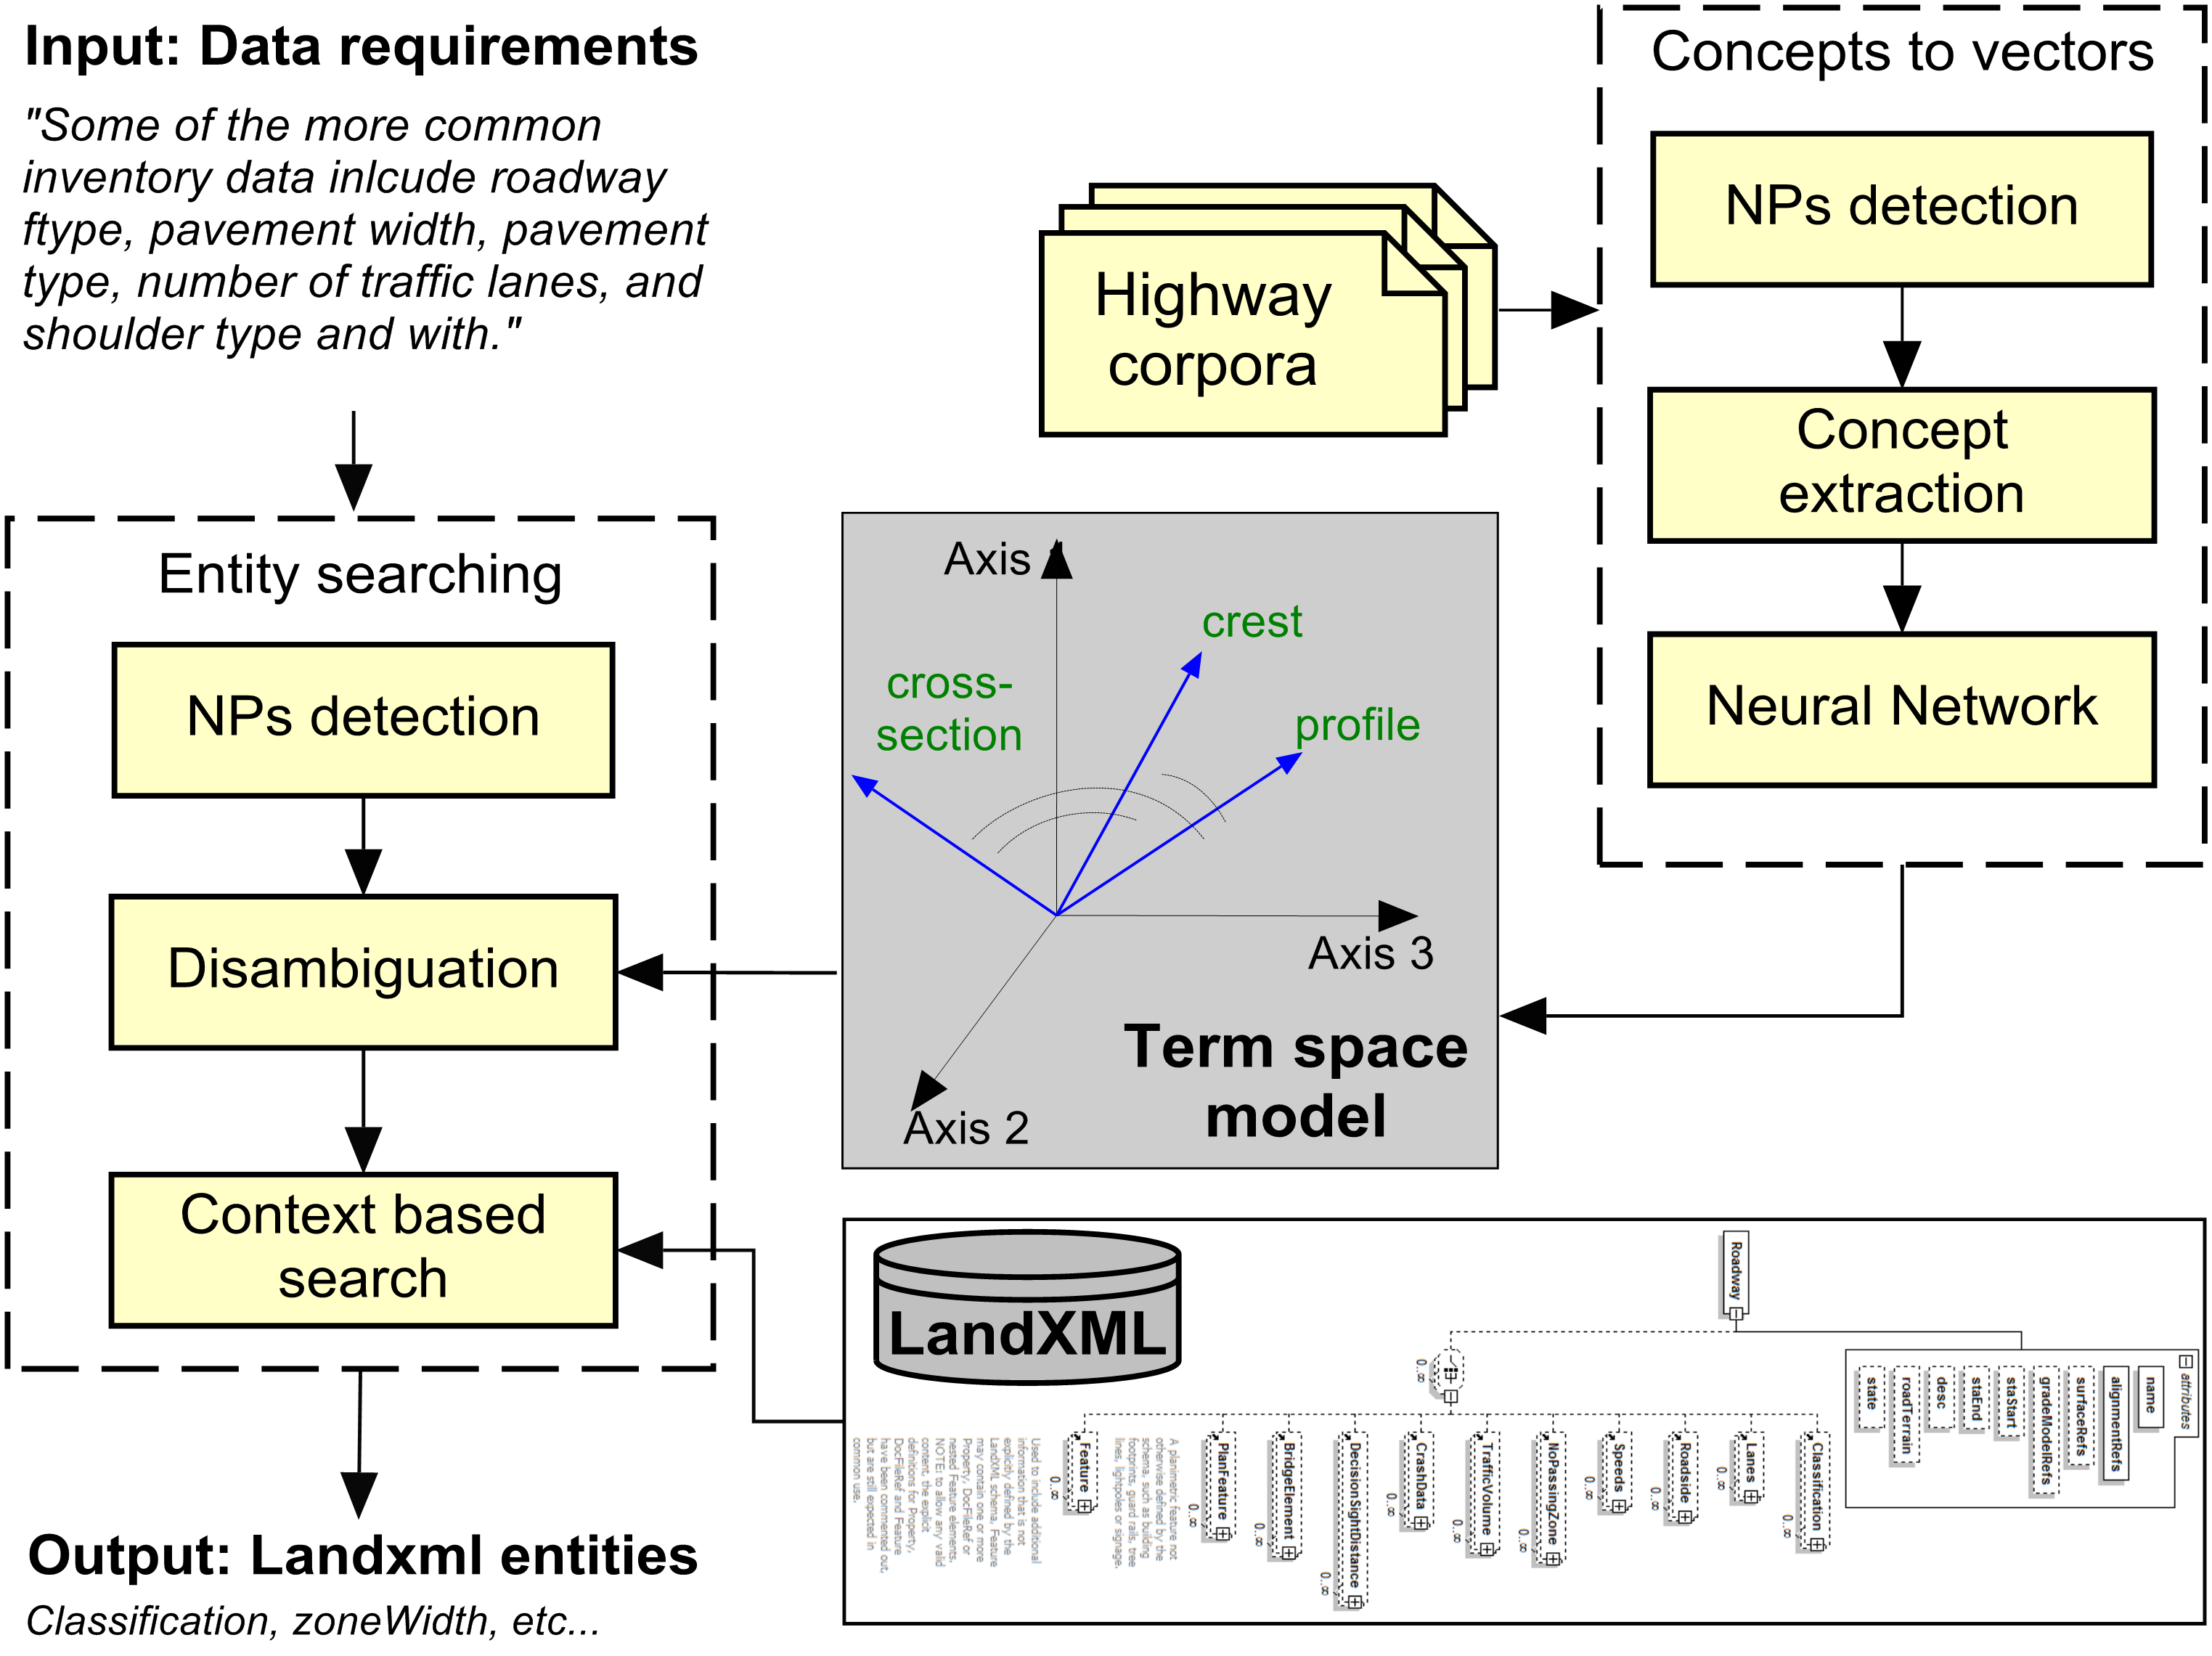
\includegraphics[width=0.67\textwidth]{framework3}
\caption{Overall architecture for automated generation of MDV}
\label{fig:framework}
\end{figure}
%
Figure \ref{fig:framework} presents the proposed method for automated generation of model views. The framework is consisted of two components that are: (1) a highway term space model, and (2) a semantic searching algorithm. The first module previously presented by the authors in, aims to extract highway related technical concepts from the highway corpora and transform concepts into vectors representing their meanings by employing a neural network (NN) model and a set of NLP techniques. In this paper, the model is extended with larger training datasets and post-processing to reorganize terms in categories which improves the semantic data searching algorithm. Using this concept vector space, synonyms or associated concepts can be determined based on the distance or angle between vectors. The purpose of the second module is to semantically search for LandXML entities and attributes based on the natural language data requirement inputs. In order to achieve this objective, NLP techniques firstly are applied on the natural language data requirements to extract keywords that representing what types of data needed to be transferred to the data receiver. A proposed algorithm then is utilized to disambiguate the meaning of extracted required data keywords based on the term space model and search for equivalent entities or attributes included in the LandXML data schema. The following sections respectively presents the process of building the highway term space model and the searching algorithm along with details on which methods/tools utilized. 
%
\section{Highway term space model} \label{sec:vector-space}
%
%introduction to the distributional vector model, fundamental theory,  the overall process to translate technical terms into vectors representations. the role of vector space allow measure the similarity between 
This section presents the extension of the H-VSM developed by the authors' previous work with the extending of training datasets and post-processing of the vector space model. The ultimate goal of this module is to build a model that can support the disambiguation task. For disambiguation, there are several methods including thesaurus based, ontology based and distributional method. The first two methods required a full lexicon or ontology including concepts description for all aspects/disciplines in the highway industry. These methods would be ideal for the disambiguation task if domain related thesauruses are available. However, since building up those dictionaries required a huge amount of empirical work, they are still limited. Wordnet \cite{miller95} which is one of the largest lexicons available containing 117,000 synsets, but it is generic and is not suitable for the highway domain. For this reason, this research employs the distribution method which is based on an unsupervised machine learning method to train unlabeled data and learn the meaning of words by analyzing the context of words. For this reason, this research employed an unsupervised machine learning method called Skip-gram, proposed by \cite{mikolov13a}, to train unlabeled data and learn the meanings of words by analysing their context words. The process of developing the H-VSM includes the following steps: (1) text document collection, (2) technical term extraction, and (3) semantic similarity training. The sub-sections below discuss the detailed procedures for each step. 
%
\subsection{Data collection}
%how to collect data, how to clean data to get them readay for training model
%aim text folow remained, flow direction. bottom down, 
%remove heading (chapter, section, subsection), footnote, numerbing, bullets, hyperlink, url, 
As mentioned earlier, the H-VSM was built using a machine learning model which use a text corpus as the training data. To support the learning of highway related technical term a highway corpus was collected in this study was built upon a number of documents from multiple sources including textbooks, and highway engineering manuals from federal Department of Transportation and from 22 state DOTs. The focus of highway corpora in this this research were on three  project phases including design, construction and asset management. Technical terms in a guidance document in the engineering field are organized in various formats such as plain text, tables, and equations. Since tables and equations are not yet supported by the state-of-the-art NLP techniques, they are removed from the text corpora. The result of data collection is a plain text corpora consisting of 16 million words. This dataset is utilized to extract highway related technical terms which are then trained and converted into vectors.
%
\subsection{Pre-processing and multi-word term candidate extraction}
%
\begin{figure}[t]
\centering
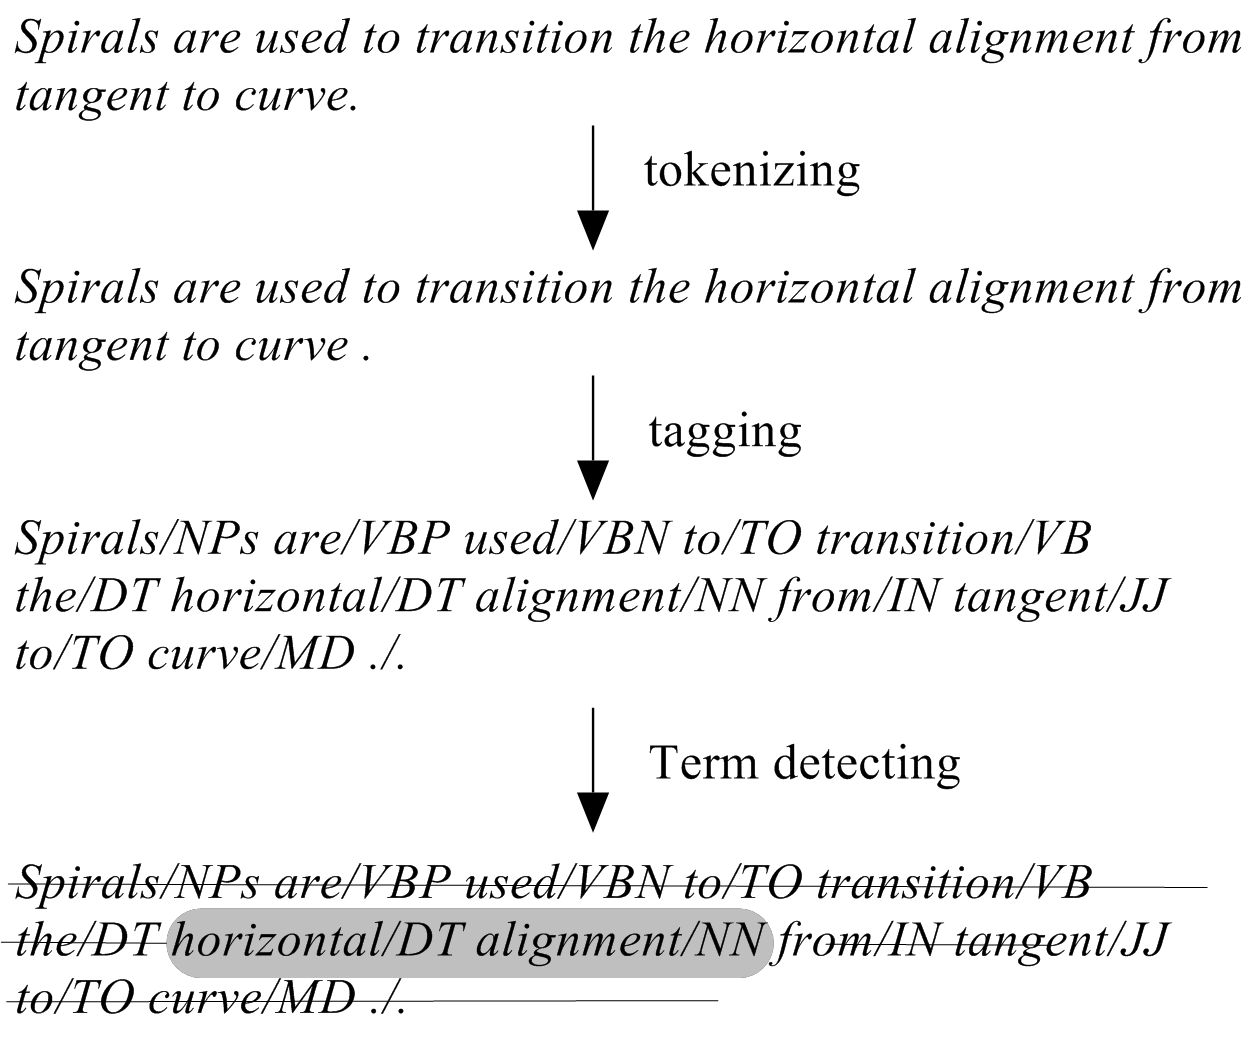
\includegraphics[width=0.45\textwidth]{NP_detecting}
\caption{Linguistic processing procedure to detect technical terms}
\label{fig:np_detect}
\end{figure}
%
The collected corpus above was processed to extract term candidates. Linguists argue that a technical term is either a noun (e.g., road) or a noun phrase (NP) (e.g., right of way) that frequently occurs in the domain text documents (Justeson and Katz 1995) \cite{justeson95}. Therefore, nouns and NPs are good term candidates. The linguistic process, as illustrated in Figure Figure \ref{fig:np_detect}. To support the generation of term candidates, a number of NLP techniques including sentence segmentation, tokenization and Part of Speech (POS) tagging will be applied on the corpus to assign tags (adjective, noun, pronoun or verb) to each of the words. The OpenNLP library is used to perform this task. The following rules, which are modified from the filters to extract multi-word terms suggested by Justeson and Katz (1995)\cite{justeson95}, will be applied to extract single-word and multi-word term candidates.
%
\begin{table} [t]
	\caption{Term candidate filters}
	\label{table:term_filter}
	\centering
	\small
	\renewcommand{\arraystretch}{1.25}
	\begin{tabular}{l l}
		\hline
		\textbf{Pattern} & \textbf{Examples}\\
		\hline
		(Adj|N)*N		& road, roadway shoulder, vertical alignment\\
		(Adj|N)*N Prep (of/in) (Adj|N)*N	&	right of way, type of roadway\\
		(Adj|N)* 'and/or' (Adj|N)*N & vertical and horizontal alignment\\
		\hline
		\multicolumn{2}{l}{\textit{Note:} |, * respectively denotes 'and/or', and 'zero or more'.  } \\
		\hline
	\end{tabular}
	
	\normalsize
\end{table}
% 
\par
The first two filters directly detect noun phrases that occur separately, and the third filter is to count for cases where multiple terms are represented in conjunctions (e.g., ='vertical and horizontal alignment'). For each instance of conjunction, an extra processing will be applied to break it into individual terms. For example, the conjunction 'vertical and horizontal alignment' will become 'vertical alignment' and 'horizontal alignment'. This division process determines the main part ('alignment') which is shared by two terms and the dependent parts ('vertical' and 'horizontal'). This research will use the Stanford Dependencies Parsing tool , which is able to analyze dependencies between sentiment units, to split conjunctions phrases into separate phrases.  
\par
In order to avoid the distinguishing between syntactic variants of the same term, for example 'roadway' and 'roadways', term variants will be normalized. The following are three types of syntactic variants and the proposed normalization methods. 
\begin{itemize}
	\item Type 1 - Plural forms, for example 'roadways' and 'roadway'. The Porter stemming algorithm (Porter 1980) \cite{porter80}, which can assist the automated removal of suffixes will be applied on the corpus before extracting NPs.
	\item Type 2 - Preposition noun phrases, for example 'roadway type' and 'type of roadway'. In order to normalize this type of variant, the form with preposition needs to be converted into the non-preposition form by removing the preposition and reverse the order of the remaining portions. For example, 'type of roadway' will become 'roadway type'.
	\item Type 3 – Abbreviations, such as AADT. A linguistic rule-based method suggested by Nenadic et al. (2002) \cite{nenadic02} will be used to determine the full term for each abbreviation. This method suggested the following abbreviation definition patterns: (1) left definition pattern – NP (Abbreviation), for example Annual Average Daily Traffic (AADT); and (2) right definition pattern - (Abbreviation) NP, for example (AADT) Annual Average Daily Traffic.
\end{itemize}
\par
The candidates with the frequency below the threshold of 50 were discarded from the list.
%
\subsection{Multi-word term candidate raking and selection}
Multi-word term definition varies between authors. in this research multiple term refers to noun phrases consiting of multiple words inwhich their meaning is not simply cobining meaning from their individual words. and there a lack of formal rules for defining multi-word term \cite{frantzi20}. The termhood, which represents the degree that a linguistic unit is a domain-technical concept, of the extracted candidates will then be computed based on their frequencies in the corpus; and the top candidates will be selected. There are a number of methods for termhood evaluation such as TF-IDF (Sparck 1972; Salton and Buckley 1988) \cite{sparck72,salton88}, C-Value (Frantzi et al. 2000) \cite{frantzi20}, Termex (Sclano and Velardi 2007) \cite{sclano07}. Among these methods, Termex outperformed other methods on the Wikipedia corpus, and C-Value was the best on the GENIA medical corpus (Zhang 2008) \cite{zhang08}. This result indicates that C-value method is more suitable for term extraction from a domain corpus rather than a generic corpus. For this reason, the C-value has been widely used to extract domain terms in the biomedical field (Ananiadou et al. (2000) \cite{ananiadou20}, Lossio-Ventura et al. (2013) \cite{lossio13}, and Nenadic et al. (2002) \cite{nenadic02}). Since the corpus used in this research will be mainly collected from technical domain documents, thus C-value would be the most suitable for termhood determination. The C-value measure, as formulated in Equation \ref{eq:cvalue}, suggests that the longer a noun phrase is, the more likely that is a term; and the more frequently it appears in the domain corpus, the more likely it will be a domain term.
% 
\begin{equation}
C-value(a)=
\begin{cases}
log_2|a|.f(a), & \text{if a is not nested} \\
log_2|a|(f(a)-\frac{1}{P(T_a)}\sum_{b\in T_a} f(b)), & \text{otherwise}
\end{cases}
\label{eq:cvalue}
\end{equation}
%
where:
\begin{description}
	\item[a] is a candidate noun phrase
	\item[f] is the frequency of a in the corpus
	\item[Ta] is the set of extracted noun phrases that contains a
	\item[P(Ta)] is the number of these candidate terms.
\end{description}
\par
%Since the original C-value measure (Equation \ref{eq:cvalue}) is not able to compute termhood for single-word terms, this research will adapt the modified C-value measure (Nakagawa and Mori 2003) \cite{nakagawa03}, that replaces the |a| component with (|a|+1) to avoid the zero value in the case of single-word term.
To calculate the recall value, expert is required to final all true terms from the corpus \cite{frantzi20}. with the large corpus in this research, it is impossible to do this task. 
\par
The ranked list of term candidates will be further refined; and only ones that have C-value greater than a threshold value will be accepted as technical terms. The selection of this boundary value will be evaluated using the precision and recall measures (see Equation 2 and 3). Precision shows the percentage of correctly extracted terms in the extracted list; and recall measures the percentage of technical terms in the corpus that are extracted. Experts in the highway industry will be invited in the evaluation phase to determine if a technical term is correctly recognized; and based on this, precision and recall values will be determined. The priority in this research is to minimize the number of missing domain terms (high recall), thus the threshold value will tend to be low. However, if the term list gets longer, there is a higher chance that non-technical terms are selected (low precision). Thus, domain experts’ opinion will be used to determine a threshold value that balances between these two criteria. 
%
The list of extracted ranked candidate with the c-value below the value of 0 was discarded from the list which was then manually evaluated true terms and non-terms. term would provide information for a certain concepts. for example, project location, this is a compound phrases of project and location, would provide one attribute of project is location. 
%
result: 8922 terms with c-values greater 0. 
\begin{table} [t]
	\caption{Examples of extracted terms and evaluation}
	\label{table:term_evaluation}
	\centering
	\small
	\renewcommand{\arraystretch}{1.25}
	\begin{tabular}{l l l}
		\hline
		\textbf{Term} & \textbf{Termhood} & \textbf{real term?}\\
		\hline
		sight distance		& 9435.314 & yes\\
		design speed & 9052.556 & yes \\
		additional information & 1829.0 & no\\
		typical section & 1801.0  & yes\\
		basis of payment & 1762.478 & no\\
		\hline
	\end{tabular}
	
	\normalsize
\end{table}

\begin{figure}[t]
	\centering
	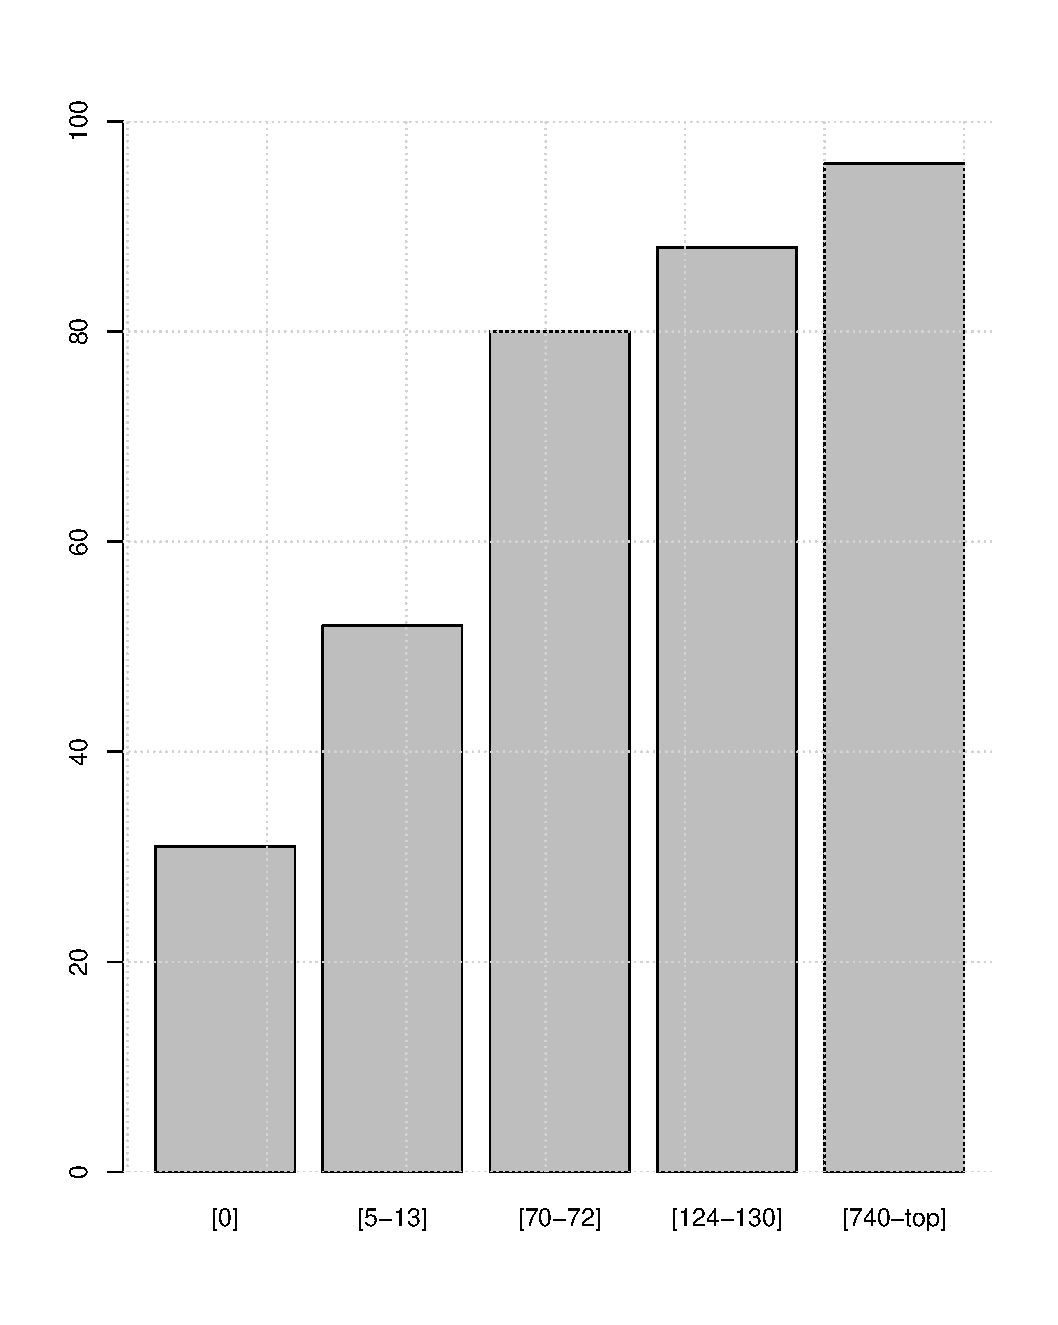
\includegraphics[width=0.45\textwidth]{term_extraction_precision}
	\caption{Precision of term extraction}
	\label{fig:term_precision}
\end{figure}

\subsection{Preparing training dataset}
The tagged and stemmed text corpora resulted from Task 1 will be reused in this task to serve as a data source for developing the semantic similarity model. The Skip-Gram model requires a set of training data in which the input data is a linguistic unit (word or term) and the output data is a set of context words. In order to collect this training dataset, the unannotated text corpora will be scanned to collect instances of terms and their corresponding context words. Each occurrence of a technical term will correspondingly generate a data point in the training dataset.
\par
Before collecting the training dataset, an additional step will be performed to handle the issue related to multi-word terms. Since document scanning is on a word-by-word basis, the corpus must be adjusted so that multi-word terms can be treated like single words. If multi-word terms are just simply replaced with unique blocks of words, the scanner will not be able to collect nested terms involved in longer terms. To allow the scanner to collect both full and nested terms, a new single unit that is compiled by connecting all individual words of a term will be added right after the last portion of the term.  In the sample sentence below, the new unique unit 'signal\_controlled\_intersection' is added after the single-word term 'intersection'.
%
\begin{center}
Before: \textit{"A signal-controlled/JJ intersection/NN depends/VB on/IN traffic/NN signals/NN..." }

After: \textit{"A signal-controlled/JJ intersection/NN signal\_controlled\_intersection/NN depends/VB on/IN traffic signals/NN…"}

\end{center}
%
The adjusted highway corpus is scanned through to find the context words for every occurrence of the technical terms in the vocabulary. The number of context words to be collected is dependent on the window size that limits how many words to the left and to the right of the target word. In the example sentence below, the context of the term 'roadway' with the context window size 10 will be the following word set {bike, lane, width, on, a, width, no, curb, gutter}. Any word in the stop list (a list of frequent words in English such as 'a', 'an', 'the' that have little meaning) will be neglected in the context set. If the target word is a multi-word term, the set of context words will not include its member words. 
\begin{center}
	"The minimum [bike lane width on a roadway with no curb and gutter] is 4 feet."
\end{center}

\subsection{Data training}
%word2vec, brief introduction about word2vec
%skip-gram model
%how to modify the method of selecting conext words
%java program

\begin{figure}[t]
	\centering
	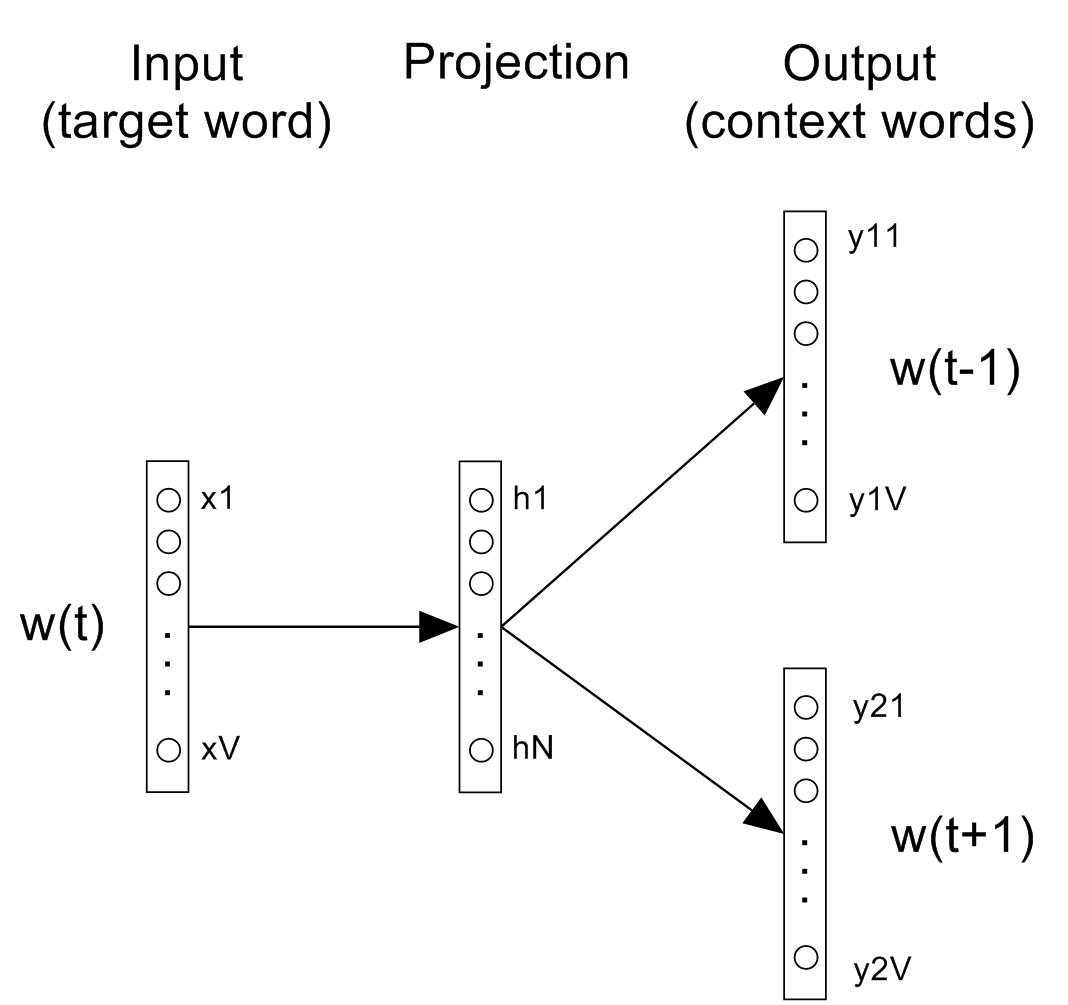
\includegraphics[width=0.45\textwidth]{skip-gram-model}
	\caption{Skip-gram model}
	\label{fig:skip-gram}
\end{figure}

The semantic similarity will be trained using the word2vec of the Apache Spark MLlib package \cite{apache16}, an emerging open-source engine, developed based on the Skip-gram neural network model (Mikolov et al. 2013) \cite{mikolov13a}. This tool includes a module that allows for automatic collection of training data from a text corpus. However, the algorithm only supports the collection of data points from single words, this module will be modified using the proposed method described in Task 2a so that multi-word terms and their nested terms can be obtained. The intended parameters used for the training model are presented in Table \ref{table:nn-parameters}. These values are mainly based on suggestions from the literature. To eliminate data points with low frequency of occurrence that are unlikely to be technical terms, word2vec includes the parameter of minimum occurrence frequency. Any vocabulary with the rate lower than the limit will be ignored. Radim Rehurek, a machine learning consultant company, suggests a range of (0-100)* depending on the data set size. Setting this parameter high will enhance the accuracy, but many technical terms will be out of vocabulary. The preliminary study based on the preliminary corpus with only several millions of words shows that with the frequency of 20, there are very few non-technical terms involved in the training dataset. Hence, with the larger dataset to be collected, this parameter can be higher and up to around 50. The second important parameter is layer size which determines the number of nodes in the hidden layer. This parameter highly affects the training accuracy and processing time. A larger layer size is better in terms of accuracy but this will be paid off by the running time. Since this research aims to develop a model that can be used for other information retrieval research, the accuracy is the first priority. This parameter may range from 10 to hundreds; in this research, it is expected to in be the range of 100-500. The final major parameter is the context window size. Google  suggests the size of 10 for the Skip-gram model. In future work, these parameters would be subject to be change so that the best model can be achieved. 
%
\begin{table} [t]
\caption{Skip-gram model parameters}
\label{table:nn-parameters}
\centering
\small
\renewcommand{\arraystretch}{1.25}
\begin{tabular}{l l}
\hline
\textbf{Parameter} & \textbf{Value}\\
\hline
Frequency threshold & 50-100\\
Hidden layer size		&	100-500\\
Context window size	&	5,10,15\\
\hline
\end{tabular}
\normalsize
\end{table}
%
Figure 3 presents the term space model developed from the training process with the parameters are 50, 300 and 10 respectively. In this model, each technical term collected from technical documents is represented as a vector in a high dimensional space; and the distance between them represents the semantic similarity. The preliminary term space presented in this paper consists of more than six thousand technical keywords. Since the vector space is a multi-dimensional space according to the size of hidden layer. In order to illustrate, present space in 2D graph, PCA (Principle component Analysis) was used to reduce the size to 2 dimensions. 
%
\begin{figure}[t]
	\centering
	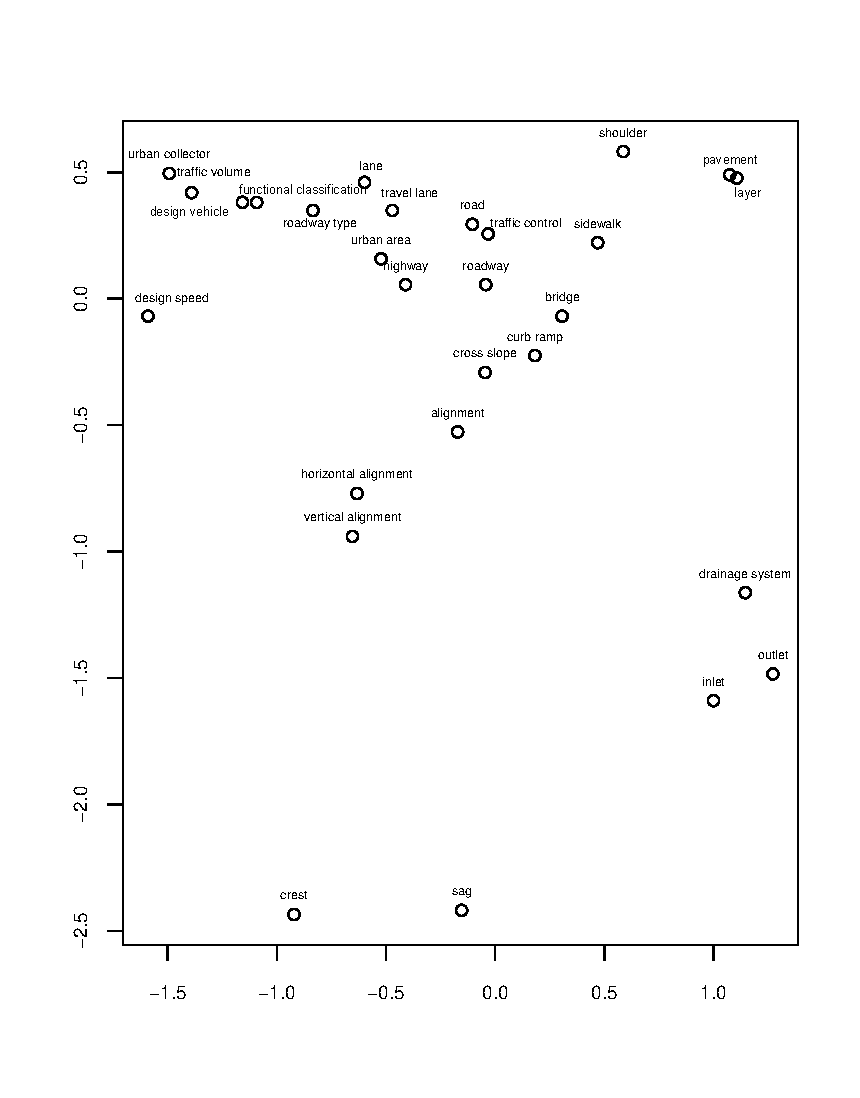
\includegraphics[width=0.45\textwidth]{Rplot_space}
	\caption{Highway term space model (H-VSM)}
	\label{fig:hvsm}
\end{figure}

The similarity between terms can be measured by the angle between two work representation vectors or the distance between two word points. The following shows two measures of word sense similarity.
%
$$cosine\_similarity = \frac{A.B}{||A||.||B||}  $$
$$dis\_similarity =\sqrt{(xA_1-xB_1)^2+(xA_2-xB_2)^2+...+(xA_n-xB_n)^2} $$

Where: n is the hidden layer size.
%
\begin{table} [t]
	\caption{Examples of top nearest terms}
	\label{table:nearest_example}
	\centering
	\small
	\renewcommand{\arraystretch}{1.25}
	\begin{tabular}{l l l  l}
		\hline
		\textbf{Term} & \textbf{Nearests} & \textbf{Cosine} &\textbf{Rank}\\
		\hline
		roadway			& highway & 0.588 & 1\\
						& traveled-way & 0.583 & 2\\
						& roadway-section & 0.577 & 3\\
						& road & 0.533 & 4\\
						& traffic-lane & 0.524 &5\\
						& separating & 0.522 &6\\
						& adjacent-roadway & 0.519 & 7\\
						& travel-way & 0.517 & 8\\
						& entire-roadway & 0.513 & 9\\
						& ...&...& ...\\
						& roadway-shoulder & 0.505 & 12\\
						& roadway-cross-section & 0.491 & 18\\
						& undivided & 0.452 & 37\\
						& mainline-roadway & 0.450 & 42\\
		\hline
	\end{tabular}
	\normalsize
\end{table}

\section{Highway lexicon construction}
A knowledge base typically includes terms and relations. The specific objective of this task is to detect relations and based on that rearrange the vocabulary constructed in Task 1. The core relations of an ontology can be classified into the following types: synonym (meaning equivalence), hypernym-hyponym (also known as IS-A or parent-child relation), attribute (concept property), and association (e.g. part-of) (Jiang and Conrath 1997; Lee et al. 2013). A method integrating linguistic rules, machine learning and the term similarity model developed in Task 2 will be proposed to extract those relations. Among these relations, hypernym, hyponym and attribute can be detected independently using linguistic rules and/or statistical methods. In contrast, since synonym recognition is well known as the process of evaluating the sharing of common attributes, hypernyms, and hyponyms, this process will rely on the results from the detection of other relations. This task will first detect the following relations (hypernyms, hyponyms and attributes) and then use them as features to find synonyms.
\par
the list of semantic nearest words generated from the semantic similarity model contain a list of various type of relations. this research consider the following three groups of relations including (1) attribute, (2) hyponym and (3) synonym/sibling and functional relation. For example, in the example presented in Table \ref{table:nearest_example}, true synonyms are highway (1), traveled-way (2) or road(4); roadway-section (3), roadway-shoulder (12) are attributes of the roadway concept; and adjacent-roadway (7), undivided (37) are hyponyms which showing differnt types of roadway.Tthe following sections present the procedure followed to reorganized the extracted list of nearest words into the three categories. 
\begin{algorithm}
	\caption{Near term classification algorithm}\label{euclid}
	\begin{algorithmic}[1]
		\State \textbf{Inputs}: term \textit{t}, list of nearest terms \textit{N}, full list of terms \textit{F}
		\State \textbf{Output:}: Classified list of terms \textit{C}
		\Procedure{Term classification procedure}{}
		%\State $\textit{n} \gets \text{size of }\textit{W}$
		%\State $\textit{m} \gets \text{size of }\textit{T}$
		\State $\textit{Att} \gets \text{list of attributes}$
		\State $\textit{Hyp} \gets \text{list of hyponyms}$
		\State $\textit{Syn} \gets \text{list of synonyms}$
		\State $\textit{w} \gets \textit{null}$
		\ForAll {$n \in N$}
			\If {$n$ contains \textit{t}}
				\State $w \gets n$
	
			\Else
				\ForAll {$f \in F$}
					\If {$f$ contains both $n$ and \textit{t}}
						\State $w \gets f$	
						\State Break for

					\EndIf
				\EndFor
			\EndIf
		\EndFor
		\If {$w$ matches \textit{Attribute pattern}}
			\State add $w$ to \textit{Att}
		\ElsIf {$w$ matches \textit{Hyponym pattern}}
			\State add $w$ to \textit{Hyp}
		\Else
			\State add $w$ to \textit{Syn}
		\EndIf
		\State Cluster \textit{Syn} and discard low relevant terms

		\EndProcedure
	\end{algorithmic}
\end{algorithm}
\subsection{Attribute and hyponym patterns}
%
The list of near words consists of various types of relationships such as attribute (lane-width), hypernyms-hyponyms (roadway-facility), synonyms (sag-profile) and other functional related terms (lane-bike). The list of nearest words will be reorganize into three categories: (1) attributes, (2) hyponyms and (3) other near term. This task aims to determine the typical attributes for the highway project related concepts using a hybrid method. Attributes, also known as the ‘property-of’ relation in ontology learning, is critical to describe a real-world concept. This research will follow the method suggested by Lee et al. (2013) \cite{lee13} to extract attributional information from the highway corpus collected in Task 1. The corpus will be scanned to collect word sequences that satisfy a certain feature pattern. This research will perform an extensive review on pattern-based attribute extraction research to collect the list of feature patterns. Examples of these patterns are presented in Table 3. For example, with pattern 1, we can infer that Noun1 is a good attribute candidate of concept Noun2; and Noun2 is an attribute of Noun1 in the pattern 2. For the second group
%
\begin{table} [t]
	\caption{Patters to extract attributes}
	\label{table:attribute_pattern}
	\centering
	\small
	\renewcommand{\arraystretch}{1.25}
	\begin{tabular}{l l l}
		\hline
		\textbf{Relation} \textbf{Pattern} & \textbf{Example}\\
		\hline
		Attribute &	Noun of Target & the width of the road\\
		& Target Noun	&	road width, project cost\\
		Hypernym-hyponym & Noun Target & vertical alignment isA alignment\\
		\hline
	\end{tabular}
	\normalsize
\end{table}
%
\begin{itemize}
	\item 
\end{itemize}
%
After the candidate list is refined, the frequency of occurrence for each candidate will then be used to compute the degree that term 'a' is an attribute of concept 'c'. If 'a' is a typical attribute of 'c', it should frequently occur in the corpus. Each concept 'c' will correspondingly have a list of attribute candidates (called list A) and their frequency of occurrences. The likelihood that 'a' is an attribute of concept 'c' is estimated using the normalized probability formula (see Equation \ref{eq:attribute}). The attribute candidates for each concept will be ranked by the likelihood measure and the top list over a threshold value will be accepted as typical attributes. 
\begin{equation}
P(a|c)=\frac{n(c,a)}{\sum_{a* \in A} n(c,a)}
\label{eq:attribute}
\end{equation}

\subsection{Synonym/sibling and functional relation recognition}
the previous proposed method are used to recognize the first two group. the remain words will fall into the final group. however, this list include long list of terms. and some of them have far or even no relation with the target word. In order to address this issue, this research employed the K-mean clustering algorithm \cite{macqueen67} to divide the remaing list into multile layers based on their similarity score. the model can provide a list of nearest words and terms. this list is needed to filter to selected the most nearest ones. this research employ the k-mean clustering algorithm \cite{macqueen67} to discard unclosed terms. the nearest list is clustering into three distinguished groups based on their similarity score. the last group is removed from the nearest list.
%
\begin{table} [t]
	\caption{Examples of top nearest terms}
	\label{table:term_clustering}
	\centering
	\small
	\renewcommand{\arraystretch}{1.25}
	\begin{tabular}{l l l l l}
		\hline
		\textbf{Term}	&\textbf{Relation Group}	& \textbf{Nearests} & \textbf{Cosine} & \textbf{Rank}\\
		roadway			&Synonym					& highway & 0.588 & 1\\
						&							& traveled-way & 0.583 & 2\\
						&							& road & 0.533 & 4\\						
						&							& traffic-lane & 0.524 &5\\ 						
						&							& travel-way & 0.517 & 8\\  \cmidrule{2-5}
						&Attribute					& separating & 0.522 &6\\
						&							& roadway-section & 0.577 & 3\\						
						&							& roadway-shoulder & 0.505 & 12\\
						&							& roadway-cross-section & 0.491 & 18\\\cmidrule{2-5}						
						&Hyponym					& adjacent-roadway & 0.519 & 7\\
						&							& entire-roadway & 0.513 & 9\\
						&							& undivided & 0.452 & 37\\
						&							& mainline-roadway & 0.450 & 42\\
		\hline
	\end{tabular}
	\normalsize
\end{table}


\section{Evaluation} \label{sec:val}
An evaluation experiment was conducted to evaluate the context-aware searching algorithm. In this experiment, a graduate student was asked to read a randomly selected document which contains data requirements for a specific data transaction. The duty of the student was to manually identify a set of Landxml entities that would fulfill the data requirements. Meanwhile, a prototype built upon the developed algorithm was applied to automatically generate the subset of data from the same document as the student used. The results from the two methods were used to calculate the accuracy of the searching algorithm.

in order to evaluate the performance of the hvsm model in most related term searching task, this research utilized the intrinsic evaluation method which is based on the comparison between computational algorithm and a gold standard. gold standard is a manually developed dataset of word synonyms or sharing common characteristics. there are several gold standards for evaluating semantic similarity tasks such as WordSim(WS)-353 \cite{finkelstein01}, MEN \cite{bruni12} and SimLex-999 \cite{hill14}. Of these, SimLex is the nearest to this research evaluation purpose since it provide predefined list of synonyms while the latter datasets generic similarity including functional relations bothm similarity and relatedness. correlation between algorithm and human assigned rating However, these standards consist no technical terms in the highway section. This research propose the proprietary gold standard that can be used for evaluating highway specific term similarity task.the gold stand was developed based on the glossary of some technical terms in the highway section provided by Wikipedia. The glossary was inspected and final list of terms were selecting excluding terms that have no synonyms. the gold standard here include both synonym set and sibling, or hypernym-hyponym. this glossary provided plain text explanation for each term and their synonyms. the final sample of the gold stand consist of 73 terms (both signle and multi-word terms).  the automatically indentified synonyms which is the top nerest word in the indentified synonym list from the algorithm was compared with the true synonyms in the gold standard dataset. the results are measured using the following three measures including recall, precision and f-measure. the evaluation result is presented in the table \ref{table:synonym_eval}.
%
\begin{align} 
&Recall = \frac{\text{number of correctly matched concepts}}{\text{total concepts}}  \\ 
&Precision = \frac{\text{number of correctly matched concepts}}{\text{total matched concepts}}  \\
&F-measure = \frac{2.Precision.Recall}{Precision+Recall}
\end{align}
%
\begin{table} [b] 
\caption{Evaluation result}
\label{table:synonym_eval}
\centering
\small
\renewcommand{\arraystretch}{1.25}
\begin{tabular}{l l l l }
\hline
\hline
 \textbf{Model} & \textbf{Precision (\%)}  & \textbf{Recall(\%)} & \textbf{F (\%)}\\
 \hline
	\underline{50}-300-15	& 80 	& 42 	& 55\\
	\underline{75}-300-15	&-		&-		&-\\
	\underline{100}-300-15	&-		&-		&-\\
	\hline
	100-\underline{100}-15	&-		&-		&-\\
	100-\underline{200}-15	&-		&-		&-\\
	100-\underline{300}-15	&-		&-		&-\\
	\hline
	100-300-\underline{5}	&-		&-		&-\\
	100-300-\underline{10}	&-		&-		&-\\
	100-300-\underline{15}	&-		&-		&-\\

\hline
\hline
\end{tabular}
\normalsize
\end{table}

%
Table \ref{table:synonym_eval} shows the evaluation result. As presented in the table, the system shows a 90 percent precision. However, the recall is relatively low accuracy, this is possibly due to the the training data size. Since the searching algorithm accuracy is highly rely on the a capacity of finding synonyms which is based on the vector space model. This model currently is based on the data training set consisting of only 10 million words. In order to enhance the accuracy, the data training set needs to be extended. Future research will be conducted to extend the training data set. 
%
compared to the previous publication by the authors, this algorithm has been improved with significantly higher accuracy. the post-processing is one reason for the outperformance of the proposed method. 
%
\section{Conclusions} \label{sec:conclns} 
Digital data has been widely generated through the project life cycle. However, the data collected and generated in previous stages are no reusable in the downstream phases. This issue is due to the interoperability when digital data from one partner is not readable or correctly understandable by the data receiver. This research develops an framework that semantically searches for desired data from the transferred data file. The framework is composed of two components including (1) a terms space model which represents highway related concepts extracted from the highway corpora in vectors and (2) a context based searching algorithm that can search for entities in the Landxml schema based on their similarity of attributes instead of string based similarity. 
\par
The framework has been evaluated by testing on a randomly selected set of input data. The result shows the accuracy of over 80 percent. The accuracy is low due to the size of the training data. Future research will be conducted to increase the data size. 
\par
This method is broad and can be applied to other business processes such as green building checking, environment checking, etc. The method is expected to significantly improve the existing ad-hoc method of model view definition development and in return leads the the removal of this bottle neck which is restricting the seamless data integration and exchange across phases of a highway construction project.

Digital project data is now widely available throughout the project life cycle in the civil infrastructure sector. However, the data collected and generated in early project development stages are not typically reusable in the downstream phases. This is due to the interoperability issue when digital data from the original data creator is not readable or correctly understandable by the data receiver. This research developed a framework that semantically searches for the desired data from a transferred data file. The framework is composed of two components including (1) a terms space model which represents highway related concepts extracted from the highway corpora in vectors and (2) a searching algorithm that can search for entities in the Landxml schema based on their semantic similarity instead of string based similarity. 
The framework was evaluated by testing on a randomly selected set of input keywords. The result shows the accuracy of over 30 percent. The accuracy is low due to the size of the training data. Future research will be conducted to increase the data size. 
This method is broad and can be applied to extract data supporting for various business processes such as green building checking, environment checking, etc. The method is expected to significantly improve the existing ad-hoc method of model view definition development and in return leads the removal of this bottle neck that is restricting the seamless data integration and exchange across phases of a highway construction project.
 

%bibliography
\bibliography{2nd_paper_bib}
%
%
\end{document}

